\documentclass[aip, cp, amsmath, amssymb, reprint]{revtex4-2}

\usepackage{graphicx}
\usepackage{dcolumn}
\usepackage{bm}

\input{preamble/preamble}
\input{preamble/tikz}
\input{preamble/macros}


% ========================================= %
% LaTeX Template by Aditya K. Rao
% Contact at adi.rao@mail.utoronto.ca

% Change for each document [!!!]
\newcommand\course{PHY385}	% Course Code [!!!]txt
\newcommand\doctitle{Michael Interferometer} % Report Title [!!!]
\newcommand\firstauthorname{Aditya K. Rao}
\newcommand\firstauthorstdnum{Student Number: 1008307761}
\newcommand\firstauthoremail{adi.rao@mail.utoronto.ca}
%\newcommand\secondauthorname{Author Two}
%\newcommand\secondauthorstdnum{Student Number: 0000000000}
%\newcommand\secondauthoremail{report.author@mail.utoronto.ca}
\newcommand\advname{Boris Braverman\space} % Advisor Name [!!!]  
\newcommand\taname{Michael Sloan\space} % Advisor Name [!!!] 
\newcommand\lponename{Jack Wang\space}
\newcommand\lptwoname{Yiheng Wang\space}  
\newcommand{\location}{MP222} % Location [!!!]
% ========================================= %
 
% ============== EQUIPMENT ================ %

\newcommand{\oscope}{\texttt{DSOX1202G}\space}
\newcommand{\pdiode}{\texttt{DET36A2}\space}
\newcommand{\hene}{\texttt{HNLS008L}\space}

% ========================================= %



%\pagenumbering{gobble}
\usepackage{listings}

\renewcommand\lstlistingname{Code Reference}
\renewcommand\lstlistlistingname{Code Reference}
\usepackage{tikz}
\usetikzlibrary{patterns}

\usepackage{circuitikz}

%\addbibresource{references.bib}
\usepackage{lipsum}
\usetikzlibrary{calc}

\begin{document}
\onecolumngrid
\pagenumbering{arabic}
\title{\doctitle}
\author{\firstauthorname}
\email{\firstauthoremail}
\thanks{\firstauthorstdnum}

\author{\lponename}
\author{\lptwoname}

%\email{report.author@mail.utoronto.ca}
%\thanks{Student Number: 0000000000}
\affiliation{
University of Toronto \\
\location, 60 St. George Street, Toronto, Ontario M5S 1A7, Canada.% Force line breaks with \\ if necessary
}

\date{\today} %Put in date of submission [!!!]

\preprint{APS/123-QED}
\begin{abstract}
    An experiment to observe effect of variations of path length in a Michaelson Interferometer was designed. It was theorized that variations in the path length difference would result in variation in the interference pattern observed. This is due to the direct relationship between the time delay between the two beams and the path differnce in each arm of the interferometer. Due to difficulties in the experimental setup, no significant data was obtained. However, the expected results and techcniques are discussed. Moreover, the influence of the polarization of the light in each arm of the interferometer was discussed. It was suggested that the addition of a quarter waveplate would result in an asymmetric interference pattern.
\end{abstract}
    \maketitle
    %\tableofcontents 

    \lhead{\firstauthorname\vspace{0.1cm}}
    \chead{\textbf{\course} \\ \doctitle}
    \rhead{\textbf{Prof:} \advname \\ \textbf{TA:} \taname}
    \nocite{*}

    %\newpage
    \twocolumngrid
    \section{Introduction}
        Invented by Albert Abraham Michelson 1887 \cite{pwoptics}, the Michaelson Interferometer is a configuration of mirrors and beam splitters which can be used to quantify the interference patterns of light. It has been instrumental in the development of quantum mechanics and the theory of relativity. The Michaelson Interferometer is used in a variety of applications, including the famous Michaelson-Morley experiment which was used to disprove the existence of the luminiferous aether \cite{pwoptics}.

        Michaelson Interferometers work on the basic principle of interference. In the experimental setup, a beam of light is split into two paths by a 50:50 beam splitter. Each beam travels a certain distance down each arm of the interferometer before being reflected back by a mirror at the end of the arm. These two beams are then reflected by mirrors and recombined at the beam splitter interfereing with each other. 

        This interference pattern can be manipulated by changing the path length of one of the arms. The difference in the distance travelled in each arm, $d$, will result in a time delay, $\tau$, between the two beams. The value of $\tau$ can be calculated using \eqref{eqn:timedelay}.
        
        \begin{equation} \label{eqn:timedelay}
            \tau = \dfrac{d}{c}
        \end{equation}
        
        This time delay will manipulate the points of constructive and destructive interference. The resultant change in intensity is given by \eqref{eqn:intensity}.
       
        \begin{equation} \label{eqn:intensity}
            I = 2 I_0 \left[1 +  \cos(\omega \tau)\right]
        \end{equation}

        Where $I_0$ is the intensity of the incident beam, $\omega$ is the frequency of the beam, and $c$ is the speed of light. The observed interference pattern will be a familar range of light and dark fringes eminating from the center point of the beam. The fringe contrast, $F$, is a measure of the visibility of the fringes and is calculated using \eqref{eqn:fringeconstrast}.
    
        \begin{equation} \label{eqn:fringeconstrast}
            F = \dfrac{V_{\text{max}} - V_{\text{min}}}{V_{\text{max}} + V_{\text{min}}}
        \end{equation}

        Where $V_{\text{max}}$ and $V_{\text{min}}$ are the maximum and minimum observed voltages from the photodiode, respectively. Given the realtion between intensity and voltage, one would can use the Frigne contrast to quantify the interference pattern observed. Using \eqref{eqn:fringeconstrast} with \eqref{eqn:intensity} one can relate the observed interference pattern to the intensity of the beam as the intensity is directly related to the observed voltage.

        \begin{equation} \label{eqn:fringe-vis}
            F = \frac{\text{max}(I) - \text{min}(I)}{\text{max}(I) + \text{min}(I)}
        \end{equation}

    \section{Methodology}
        The experiment was setup in accordance with the schematic in \figref{fig:setup}. The first components added to the setup were the \hene laser, and the initial two mirrors. Great care was taken to ensure that the resultant incident beam was output at an angle of incidence $\theta_i = 90\pm 1^\circ$ to the beam splitter. 

        Mirror \texttt{M2} was then attached to a translation stage and palced $10.0\pm0.5\,\text{cm}$ from the base of the beam splitter. Prior to adding the beam splitter and \texttt{M1}, the laser was turned on with all mirrors being adjusted until the back reflection of the laser was incident on the laser itself. The beam splitter, \texttt{M1} (similarly $10.0\pm0.5\,\text{cm}$), and \pdiode photodiode where then added to the setup. A shroud was placed on the photodiode lense mount to reduce the effect of ambient light. 
        
        Each component was carefully aligned to ensure that the beam was incident on the photodiode. 

        \begin{figure}[H]
            \centering
            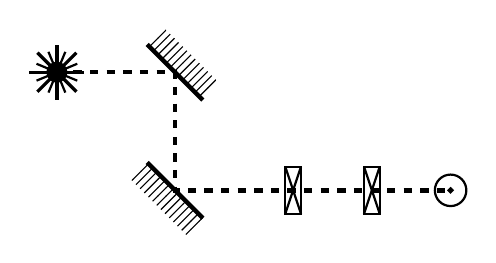
\begin{tikzpicture}
    \coordinate (L) at (0,0);
    \coordinate (M1) at (1.5,0);
    \coordinate (M2) at (1.5,-1.5);
    \coordinate (P1) at (3,-1.5);
    \coordinate (P2) at (4,-1.5);
    \coordinate (D) at (5,-1.5);

    % Laser Symbol
    \begin{scope}[scale=0.7]
        \draw[ultra thick, fill = black] (0,0) circle (0.15);
        \draw[rotate=0, very thick] (-0.5,0) -- (0.5,0);
        \draw[rotate=90, very thick] (-0.5,0) -- (0.5,0);
        \draw[rotate=45, very thick] (-0.5,0) -- (0.5,0);
        \draw[rotate=135, very thick] (-0.5,0) -- (0.5,0);

        \draw[rotate=22.5, thick] (-0.4,0) -- (0.4,0);
        \draw[rotate=67.5, thick] (-0.4,0) -- (0.4,0);
        \draw[rotate=112.5, thick] (-0.4,0) -- (0.4,0);
        \draw[rotate=157.5, thick] (-0.4,0) -- (0.4,0);
    \end{scope}


    % Mirror #1
    \begin{scope}[shift={(M1)}, rotate=-45]
        \draw[ultra thick] (-0.5,0) -- (0.5,0);
        \fill[pattern=north east lines] (-0.5,0) rectangle (0.5,0.30);
        %\coordinate (M1) at (0,-0.15);
    \end{scope}

    % Mirror #2
    \begin{scope}[shift={(M2)}, rotate=135]
        \draw[ultra thick] (-0.5,0) -- (0.5,0);
        \fill[pattern=north east lines] (-0.5,0) rectangle (0.5,0.30);
        %\coordinate (M2) at (0,-0.15);
    \end{scope}

    % Polarizer #1
    \begin{scope}[shift={(P1)}, scale=0.5]
        \draw[thick] (-0.2,0.6) rectangle (0.2,-0.6);
        \draw[thick] (-0.2,0.6) -- (0.2,-0.6);
        \draw[thick] (0.2,0.6) -- (-0.2,-0.6);
        %\coordinate (P1) at (0,0);
    \end{scope}

    % Polarizer #2
    \begin{scope}[shift={(P2)}, scale=0.5]
        \draw[thick] (-0.2,0.6) rectangle (0.2,-0.6);
        \draw[thick] (-0.2,0.6) -- (0.2,-0.6);
        \draw[thick] (0.2,0.6) -- (-0.2,-0.6);
        %\coordinate (P2) at (0,0);
    \end{scope}

    % Detector
    \begin{scope}[shift={(D)}, scale=0.5]
        \draw[thick] (0,0) circle (0.4);
        \draw[thick, fill=black] (0,0) circle (0.05);
        %\coordinate (D) at (0,0);
    \end{scope}

    % Laser Path
    \draw[ultra thick, dashed] (L) -- (M1) -- (M2) -- (P1) -- (P2) -- (D);
\end{tikzpicture}
            \caption{Schematic of experimental setup. The plano-convex lens was only added for the magnification of the fringe pattern and was not present for the initial setup. Similarly, the half wave plate would only be present for certain experiments.}
            \label{fig:setup}
        \end{figure}

        Fine and course grain adjustment to ensure interference of the incident and reflected beam was achieved using the following technique \footnote{This technique was suggested and demonstrated by the Teaching Assistant.}. First, the vertical and horizontal knobs on M1 were adjusted such that the beam is resolved just past the the photodiode. Subsequent similar adjustments were made to M2 so that the beams overlapped on the photodiode sensor.

        To magnification of the fringe pattern was achieved bv passing the input beam was passed through a plano-convex lens with a focal length of $f=25mm$ \cite{thorlabs}. The lens was placed at a distance of $f$ from the beam splitter.

        Readings were obtained via measuring the maximum and minimum observed voltages from the \pdiode photodiode. Uncertainties were quantified through the variance in the observed voltages over repeated measurements. This would be somewhat significant given that the setup is sensative to deviations in the alignment of the mirrors, beam splitter, and even varaiations in air pressure \cite{labmanual}.

    \section{Results \& Analysis}
        Despite repeated attempts, the experiment was unsuccessful in obtaining a clear interference pattern. Vibrations and resultant alignment issues caused no clear data to be obtained. Regardless, the data, should it have been obtained, would have been analyzed as follows.

        One would expect the fringe pattern to correspond with the intensity of light as defined by \eqref{eqn:intensity}. The fringe contrast would be calculated using \eqref{eqn:fringeconstrast}. 

        In accordance with \eqref{eqn:timedelay}, varying the arm length, $d$ would result in a corresponding change in the time delay, $\tau$. Then, the observed interference pattern would be different.

        The frequency of the \hene laser is a known value \cite{henemanual} and can be calculated as $\omega = \frac{c}{632.8\,\text{nm}} = 473\,\text{KHz}$. The resulting relation between $I_0$ and $d$ can then be plotted as in \figref{fig:fringe}.

        \begin{figure}[H]
            \centering
            \includegraphics[width=0.45\textwidth]{figures/PathDiffI0.png}
            \caption{Expected fringe pattern as a function of arm length as calculated in units of the incident intensity, $I_0$ of the beam. Notice points of evenetual constructive and destructive interference.}
            \label{fig:fringe}
        \end{figure}


    \section{Discussion}
        Though no significant experimental data was conducted, a discussion can still be had surrounding the speculated results and sources for uncertainty. Firstly, for the experiment to be successful, the setup would have to be conducted in a more controlled environment. The vibrations (for instance, from other groups) and difficulties with alignment significantly delayed the collection of data. 

        From figure \ref{fig:fringe}, one can see that interrogating the path difference of the Interferometer has a direct effect on the intensity of the observed interference pattern and hence will have a direct effect on the fringe contrast. The primariy source of uncertainty in such an experiment would be the alignment of the mirrors and beam splitter. However, other sources of uncertainty, such as fluctiations in the incident intensity, can be quantified directly by the variance in the observed voltages without any changes in path difference.

        Moreover, the adjustment of the translation stage has an inherent uncertainty of $\pm 0.5\,\text{mm}$ (using the readings on the micrometer) which would directly affect the path difference and hence the observed interference pattern would deviate from the expected interference pattern.

        It is also worth noting that the polarization of the light in each arm of the interferometer would have a significant effect on the observed interference pattern. If the polarizations in each arm are orthogonal, then no intereference pattern would be observed as the beams would have no common component to interfere with.

        Similarly, adding a quarter waveplate may have an interesting effect on the resulting interference pattern. Specifically, there would be difference regions of constructive and destructive interefrence leading to an asymmetric interference pattern. To make the result more extreme, one should place a linear polarizer after the interferometer as adding it before would only reduce the initial intensity of the beam, not make the effect of the waveplate more extreme
    
    \section{Conclusion}
        Two experiments were proposed and setup to investigate the relation between the path difference in two arms of a Michaelson Interferometer. Both experiments utilized a \hene laser with the resulting interefrence pattern measured by a \pdiode photodiode. 

        Results were quantified using the Frince contrast, $F$. Due to difficulties with experimental setup, for instance, alignment and environmental factors, no significant data was obtained. However, the expected results and uncertainties were discussed. It is presumed that variaations in the path difference would have a direct effect on the observes interference pattern as manipulation of the path difference would result in a change in the time delay between the two beams.

        Moreover, the polarization of the light in each arm of the interferometer would have a significant effect on the observed interference pattern. If the polarizations in each arm are orthogonal, then no intereference pattern would be observed as the beams would have no common component to interfere with. This idea may be explored further through the second proposed experiment in which a Quarter Waveplate is added to the setup. 

        By adding a quarter waveplate, one would expect to see an asymmetric intereference pattern due to contrucrive and destructive interefernece happening in different places of the beam. 


    % Line to seperate report content from acknowledgements and references
    \onecolumngrid
    \begin{center}
        \vspace{0.8cm}
        \noindent\rule{0.9\textwidth}{0.5pt}
    \end{center}
    \begin{acknowledgments}
        The work conducted by the other lab partners was instrumental in this lab. Thank you to \lponename and \lptwoname for their help in setting up the equipment and conducting the experiments. Additionally, I would like to greatly thank Teaching Assistant \taname for his guidence both during the lab and even more so on how to write the report without a full set of data. Finally, I would like to thank Professor \advname for their guidance and support through the labs and course thusfar.
    \end{acknowledgments}

\bibliography{references}

% \appendix
% \section{Appendix}
% \subsection{Raw Data}

% \subsection{Analysis Code}
% \subsubsection{Toolkit}
% \lstinputlisting{../toolkit.py}

\end{document}